%% ===========================================================================
%%  NURBS-Maxima -- manuscript for SoftwareX (Original Software Publication)
%%  Overleaf: upload the whole folder docs/softwarex/ and compile main.tex
%%  with pdfLaTeX (elsarticle.cls and elsarticle-num.bst are built into
%%  Overleaf/TeX Live).  Figures: figures/*.pdf (vector) and figures/*.csv
%%  (plotted with pgfplots), all produced by figures/make_figures.mac.
%%
%%  Placeholders to complete are marked \todo{...} and appear in red.
%%  Delete the \todo macro definition before submission to make sure none
%%  is left (compilation will then fail on any remaining placeholder).
%% ===========================================================================
\documentclass[preprint,12pt]{elsarticle}

\usepackage[T1]{fontenc}
\usepackage[utf8]{inputenc}
\usepackage{lmodern}
\usepackage{amsmath,amssymb}
\usepackage{graphicx}
\usepackage{booktabs}
\usepackage{float}
\usepackage{tabularx}
\usepackage{array}
\usepackage{xcolor}
\usepackage{listings}
\usepackage{pgfplots}
\pgfplotsset{compat=1.17}
\usepgfplotslibrary{groupplots}
\usetikzlibrary{positioning,arrows.meta,fit,backgrounds}
\usepackage[hidelinks]{hyperref}
\usepackage{lineno}
\usepackage{orcidlink}
% \linenumbers   % uncomment for the review version if requested

\newcommand{\todo}[1]{\textcolor{red}{[#1]}}
\newcommand{\pkg}{NURBS-Maxima}
\newcommand{\code}[1]{{\ttfamily\def\_{\textunderscore\allowbreak}#1}}
\setlength{\emergencystretch}{3em}

% --- Maxima listings ---------------------------------------------------------
\lstdefinelanguage{Maxima}{
  morekeywords={load,block,for,do,thru,in,if,then,else,lambda,makelist,print,
    subst,ratsimp,factor,diff,assume,float,bfloat,fpprec,sqrt},
  sensitive=true,
  morecomment=[s]{/*}{*/},
  morestring=[b]"}
\lstset{language=Maxima,
  basicstyle=\ttfamily\small,
  keywordstyle=\color{blue!60!black}\bfseries,
  commentstyle=\color{green!40!black}\itshape,
  stringstyle=\color{red!50!black},
  columns=fullflexible,keepspaces=true,
  frame=single,framerule=0.3pt,rulecolor=\color{gray!60},
  xleftmargin=2pt,xrightmargin=2pt,
  breaklines=true,showstringspaces=false,
  literate={²}{{$^2$}}1 {≡}{{$\equiv$}}1}

\journal{SoftwareX}

\begin{document}

\begin{frontmatter}

\title{\pkg: exact, symbolic and arbitrary-precision NURBS curves, surfaces and differential geometry in the Maxima computer algebra system}

%% ---- Authors ---------------------------------------------------------------
\author[unp]{Ronald Paul Santamaria Silupu\,\orcidlink{0009-0007-2226-4815}\corref{cor1}}
\ead{rsantamarias@egresados.unp.edu.pe}
\author[unp]{Yheff Alexander Castillo Maza\,\orcidlink{0009-0005-8158-8460}}
\ead{ycastillom@egresados.unp.edu.pe}
\author[unp]{Judith Keren Jimenez Vilcherrez\,\orcidlink{0000-0002-7823-1533}}
\ead{jjimenezv@unp.edu.pe}
\author[unp]{Rubén Teodoro Urbina Guzmán\,\orcidlink{0000-0002-8544-3307}}
\ead{rurbinag@unp.edu.pe}
\author[unp]{Victor Bernardo Sosa Gonzales\,\orcidlink{0000-0002-0519-257X}}
\ead{vsosag@unp.edu.pe}
\cortext[cor1]{Corresponding author.}
\affiliation[unp]{organization={Universidad Nacional de Piura},
  city={Piura}, country={Peru}}

\begin{abstract}
\pkg{} is an open-source package for the free computer algebra system Maxima that implements the standard algorithms for non-uniform rational B-spline (NURBS) curves and surfaces together with their differential geometry. A single code base runs in exact rational and radical arithmetic, with symbolic weights, in double precision and in arbitrary-precision floating point; the type of the input selects the arithmetic. The package covers evaluation, rational derivatives, knot insertion and refinement, degree elevation, Bézier decomposition, interpolation, point inversion, fundamental forms, Gaussian, mean and principal curvatures, singular points, area, volume and total curvature, with export to VTK, STL, OBJ, CSV and NURBS-Python JSON. It is validated by 95 regression tests and a cross-validation with NURBS-Python that agrees to $2.3\times10^{-13}$.
\end{abstract}

\begin{keyword}
NURBS \sep B-splines \sep computer algebra \sep Maxima \sep differential geometry \sep arbitrary precision
\end{keyword}

\end{frontmatter}

%% ===========================================================================
\section*{Code metadata}
\label{sec:metadata}

\begin{table}[H]
\small
\begin{tabularx}{\linewidth}{@{}l>{\raggedright\arraybackslash}p{0.38\linewidth}>{\raggedright\arraybackslash}X@{}}
\toprule
Nr. & Code metadata description & Metadata \\
\midrule
C1 & Current code version & v2.0.0 \\
C2 & Permanent link to code/repository used for this code version & \url{https://github.com/ronaldpaul78/NURBS-Maxima} \\
C3 & Permanent link to Reproducible Capsule & \todo{\url{https://doi.org/10.5281/zenodo.0000000}} \\
C4 & Legal Code License & MIT \\
C5 & Code versioning system used & git \\
C6 & Software code languages, tools, and services used & Maxima language; gnuplot (graphics); Python~3 with NURBS-Python (geomdl) only for cross-validation \\
C7 & Compilation requirements, operating environments \& dependencies & Maxima $\geq$ 5.40 (tested with 5.46.0 on GCL); gnuplot; any OS supported by Maxima/wxMaxima (Windows, Linux, macOS). No compilation needed. \\
C8 & If available Link to developer documentation/manual & \url{https://github.com/ronaldpaul78/NURBS-Maxima/blob/main/docs/API.md} \\
C9 & Support email for questions & rsantamarias@egresados.unp.edu.pe \\
\bottomrule
\end{tabularx}
\caption{Code metadata.}
\label{tab:metadata}
\end{table}

%% ===========================================================================
\section{Motivation and significance}
\label{sec:motivation}

Non-uniform rational B-splines (NURBS) combine the local control of B-splines with the exact representation of conics and quadrics through rational weights~\cite{PieglTiller1987,Piegl1991,Farin1992,PieglTiller1997,Farin1999,Farin2002}. They are the geometric basis of computer-aided design (CAD) exchange and of isogeometric analysis~\cite{Hughes2005,Cottrell2009}. Mature open implementations, such as NURBS-Python (geomdl)~\cite{Bingol2019}, the MATLAB/Octave NURBS toolbox~\cite{SpinkNurbsToolbox,OctaveNurbs} on which GeoPDEs builds~\cite{deFalco2011}, and the CAD kernels, are numerical libraries: every operation is carried out in double precision and quantities such as curvature are sampled pointwise.

Three recurring research and teaching tasks need more than that:
\begin{enumerate}
\item \emph{Symbolic verification.} Proving that a rational quadratic curve is a circle, that knot refinement leaves a surface unchanged, or that a patch has a prescribed curvature requires exact arithmetic, not agreement to machine precision.
\item \emph{Closed-form design sensitivities.} A designer who varies a weight $w$ wants curvature or area as a function of $w$, not a table of samples. This requires the NURBS algorithms to run on symbolic data.
\item \emph{Ill-conditioned evaluation.} At degenerate points, such as the poles of a surface of revolution, the formulas for the Gaussian and mean curvatures divide two quantities that vanish together. Double precision loses every significant digit there; arbitrary precision does not.
\end{enumerate}

This work builds on our previous Python developments in geometric design: surfaces constructed from planar curves~\cite{Urbina2025LACCEI}, Coons surfaces expressed as B-spline surfaces~\cite{Castillo2025Coons}, NURBS surfaces generated from controlled NURBS curves~\cite{Urbina2025ICCSA}, spheres and tori of revolution as NURBS surfaces~\cite{Castillo2026ARTIIS}, swept surfaces from NURBS curves~\cite{Santamaria2026LACCEI}, and a rational parametric hypersurface studied with symbolic visualisation~\cite{Vilcamiche2025Viviani}. Those implementations work in floating point; the step taken here is to move the same constructions into a computer algebra system, where they can also be carried out exactly and symbolically.

Computer algebra systems are the natural environment for these tasks, but spline support in them is either proprietary (Mathematica~\cite{WolframBSpline}, Maple~\cite{MapleBSpline}) or, for the free system Maxima~\cite{Maxima}, absent: to our knowledge there is no NURBS package for Maxima \todo{confirm with a systematic search before submission}. Maxima, a descendant of Macsyma, is widely used in teaching through its notebook interface wxMaxima~\cite{wxMaxima}, for instance in calculus courses~\cite{Karjanto2021}. Dedicated tools for teaching or interactively modelling curves and surfaces exist~\cite{Miller2010,Peixoto2024}, but they are numerical and do not expose the algorithms to symbolic manipulation.

\pkg{} fills this gap. It implements the algorithms of Piegl and Tiller~\cite{PieglTiller1997} in pure Maxima for curves and surfaces, adds a differential-geometry layer for NURBS surfaces, and exports to the usual visualisation and exchange formats. Table~\ref{tab:comparison} positions it with respect to the tools a researcher would consider for the same tasks. The combination it offers (a free licence, NURBS objects that accept exact and symbolic data, and built-in differential geometry of rational surfaces) is, to our knowledge, not available elsewhere. geomdl remains the reference for floating-point speed and file formats, and we use it as an independent oracle in the validation.

\begin{table}[t]
\centering
\scriptsize
\setlength{\tabcolsep}{3pt}
\begin{tabularx}{\linewidth}{@{}>{\raggedright\arraybackslash}p{2.6cm}*{5}{>{\raggedright\arraybackslash}X}@{}}
\toprule
 & \pkg & geomdl~\cite{Bingol2019} & NURBS toolbox (MATLAB/Octave)~\cite{SpinkNurbsToolbox,OctaveNurbs} & Mathematica~\cite{WolframBSpline} & Maple~\cite{MapleBSpline} \\
\midrule
Licence & MIT; host GPL & MIT & GPL$^\dagger$; MATLAB host proprietary & proprietary & proprietary \\
Rational curves and surfaces & yes & yes & yes & yes$^\dagger$ & B-spline basis only$^\dagger$ \\
Exact / symbolic NURBS data & yes, all algorithms & no & no & basis only$^\dagger$ & basis only$^\dagger$ \\
Closed-form curvature in a weight & yes & no & no & not built in$^\dagger$ & not built in$^\dagger$ \\
Arbitrary precision & yes & no & no & yes$^\dagger$ & yes$^\dagger$ \\
Knot insertion, refinement, degree elevation & yes & yes & yes$^\dagger$ & not exposed$^\dagger$ & no$^\dagger$ \\
Surface curvatures $K$, $H$, $\kappa_{1,2}$, $\iint K\,dA$ & yes & no$^\dagger$ & no$^\dagger$ & generic tools$^\dagger$ & generic tools$^\dagger$ \\
Export & VTK (with $K,H$), STL, OBJ, CSV, JSON & OBJ, STL, OFF, VTK, JSON, CSV$^\dagger$ & via host$^\dagger$ & via \code{Export}$^\dagger$ & via \code{Export}$^\dagger$ \\
Algorithms readable in host language & yes & yes & yes & no & no \\
\bottomrule
\end{tabularx}
\caption{Comparison with related tools. $^\dagger$\,\todo{From general knowledge of the products; verify against current documentation before submission.}}
\label{tab:comparison}
\end{table}

%% ===========================================================================
\section{Software description}
\label{sec:description}

\pkg{} is a single Maxima source file (\code{nurbs\_maxima.mac}, about 1\,350 lines and 110 public functions) loaded with \code{load("nurbs\_maxima.mac")}. It has no dependencies beyond Maxima and gnuplot, both distributed with wxMaxima. The repository contains the package, seven worked examples, a test directory, an API reference, benchmarks and a Spanish-language teaching notebook that walks through the source.

\subsection{Software architecture}
\label{sec:architecture}

Curves and surfaces are Maxima structures, \code{nurbscrv(degree, knots, ctrlpts, weights)} and \code{nurbssrf(degree\_u, degree\_v, knots\_u, knots\_v, ctrlpts, weights)}, with indices starting at 0 as in~\cite{PieglTiller1997}. Constructors validate knot vectors (length, monotonicity, multiplicity) and weights (positive when numeric; symbolic weights are accepted). The code is organised in five layers plus a validation suite (Fig.~\ref{fig:architecture}).

\begin{figure}[t]
\centering
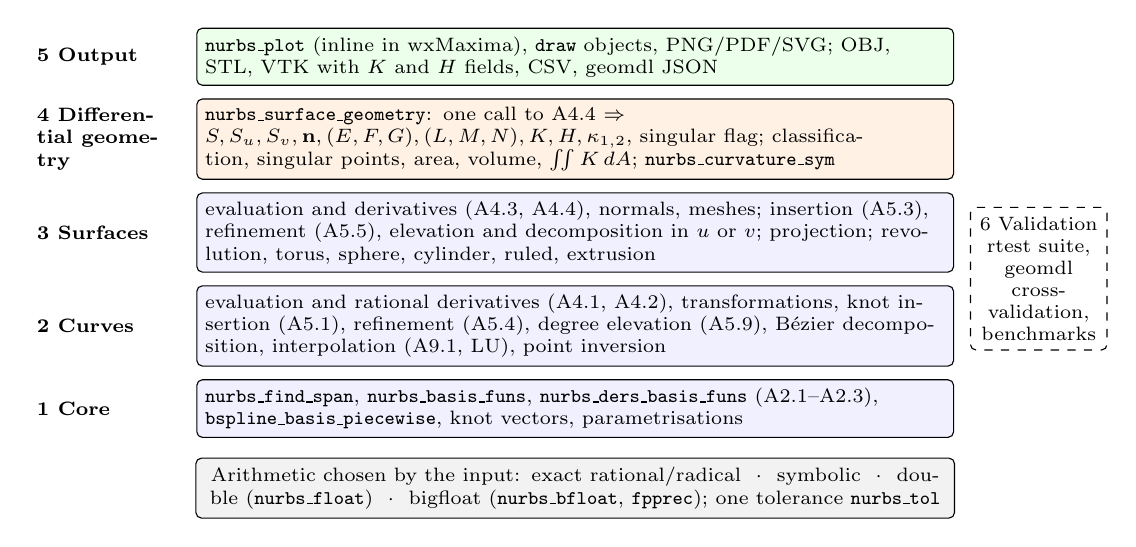
\begin{tikzpicture}[
  box/.style={draw, rounded corners=2pt, align=left, font=\scriptsize,
              text width=9.4cm, inner sep=3pt, fill=#1},
  box/.default=white,
  lab/.style={font=\scriptsize\bfseries, align=left, text width=1.7cm},
  node distance=1.6mm]
\node[box=blue!6] (core) {\code{nurbs\_find\_span}, \code{nurbs\_basis\_funs}, \code{nurbs\_ders\_basis\_funs} (A2.1--A2.3), \code{bspline\_basis\_piecewise}, knot vectors, parametrisations};
\node[box=blue!6, above=of core] (crv) {evaluation and rational derivatives (A4.1, A4.2), transformations, knot insertion (A5.1), refinement (A5.4), degree elevation (A5.9), Bézier decomposition, interpolation (A9.1, LU), point inversion};
\node[box=blue!6, above=of crv] (srf) {evaluation and derivatives (A4.3, A4.4), normals, meshes; insertion (A5.3), refinement (A5.5), elevation and decomposition in $u$ or $v$; projection; revolution, torus, sphere, cylinder, ruled, extrusion};
\node[box=orange!10, above=of srf] (dg) {\code{nurbs\_surface\_geometry}: one call to A4.4 $\Rightarrow$ $S, S_u, S_v, \mathbf n, (E,F,G), (L,M,N), K, H, \kappa_{1,2}$, singular flag; classification, singular points, area, volume, $\iint K\,dA$; \code{nurbs\_curvature\_sym}};
\node[box=green!8, above=of dg] (out) {\code{nurbs\_plot} (inline in wxMaxima), \code{draw} objects, PNG/PDF/SVG; OBJ, STL, VTK with $K$ and $H$ fields, CSV, geomdl JSON};
\node[lab, left=2mm of core] {1 Core};
\node[lab, left=2mm of crv] {2 Curves};
\node[lab, left=2mm of srf] {3 Surfaces};
\node[lab, left=2mm of dg] {4 Differential geometry};
\node[lab, left=2mm of out] {5 Output};
\node[draw, dashed, rounded corners=2pt, font=\scriptsize, align=center, text width=1.5cm,
      right=2mm of crv, yshift=6mm] (val) {6 Validation\\ rtest suite,\\ geomdl cross-validation,\\ benchmarks};
\node[draw, rounded corners=2pt, font=\scriptsize, align=center, fill=gray!10,
      below=2.5mm of core, text width=9.4cm] (arith) {Arithmetic chosen by the input: exact rational/radical $\;\cdot\;$ symbolic $\;\cdot\;$ double (\code{nurbs\_float}) $\;\cdot\;$ bigfloat (\code{nurbs\_bfloat}, \code{fpprec}); one tolerance \code{nurbs\_tol}};
\end{tikzpicture}
\caption{Architecture of \pkg. Each layer only calls the layers below it; the validation suite exercises all of them.}
\label{fig:architecture}
\end{figure}

Three design decisions shape the package.

\emph{One code base, four arithmetics.} No routine forces a numerical conversion: exact input gives exact output, floating-point input gives floating-point output, and bigfloat input gives results at the precision \code{fpprec}. Because none of the algorithms branches on the sign or size of a weight, symbolic weights flow through all of them; the constructor checks positivity only when a weight is a number. \code{nurbs\_float} and \code{nurbs\_bfloat} convert whole objects before dense sampling.

\emph{A single tolerance.} All zero tests go through one predicate that always returns \code{true} or \code{false}: a floating-point value is zero when $|x|\le$\,\code{nurbs\_tol} (default $10^{-10}$), an exact constant when \code{radcan} reduces it to 0, and a symbolic expression when \code{ratsimp} does. Singular, umbilic and planar points use relative versions of the same tolerance, for instance $|S_u\times S_v|\le \mathtt{nurbs\_tol}\cdot\max(1,|S_u||S_v|)$; the umbilic test uses $H^2-K$ rather than $\kappa_1-\kappa_2$ to avoid amplifying round-off through a square root.

\emph{A shared differential-geometry helper.} \code{nurbs\_surface\_geometry(S,u,v)} performs one second-order derivative evaluation (A4.4) and returns the point, the tangents, the unit normal $\mathbf n = S_u\times S_v/|S_u\times S_v|$, the coefficients of the fundamental forms, and
\begin{equation}
K=\frac{LN-M^2}{EG-F^2},\qquad H=\frac{EN-2FM+GL}{2(EG-F^2)},\qquad \kappa_{1,2}=H\pm\sqrt{H^2-K},
\label{eq:KH}
\end{equation}
following~\cite{doCarmo1976}. Every curvature function, the VTK exporter and the integrand of $\iint K\,dA$ are thin wrappers around it, so all of them agree on what is singular. The symbolic variant \code{nurbs\_curvature\_sym} works on the exact rational expression of one patch and uses the unnormalised normal, which keeps $K$ rational in the parameters and the weights.

\subsection{Software functionalities}
\label{sec:functionalities}

\begin{itemize}
\item \emph{B-spline core:} span search, non-zero basis functions and their derivatives (A2.1--A2.3), exact piecewise polynomials of the basis, Bernstein polynomials, clamped and uniform knot vectors, uniform, chord-length and centripetal parametrisations.
\item \emph{Curves:} evaluation and rational derivatives of any order (A4.1, A4.2), exact span expressions, weights (also symbolic), affine and projective transformations through $4\times4$ homogeneous matrices, knot insertion and refinement, degree elevation, Bézier decomposition, splitting, reversal, global interpolation with an LU solver valid in exact, double and bigfloat arithmetic, and Newton point projection; curvature, torsion, Frenet frame and arc length by Gauss--Legendre quadrature.
\item \emph{Surfaces:} evaluation and partial derivatives (A4.3, A4.4), normals, isocurves, grids and triangle meshes; knot insertion, refinement, degree elevation and Bézier decomposition along $u$ or $v$; point projection; primitives (Bézier, bilinear, extrusion, ruled, revolution, torus, sphere, cylinder).
\item \emph{Differential geometry:} fundamental forms, $K$, $H$, principal curvatures and directions, point classification (elliptic, hyperbolic, parabolic, planar, umbilic, singular), search for singular points, area, enclosed volume, total curvature $\iint K\,dA$ for Gauss--Bonnet checks, and exact $[K,H]$ on a patch.
\item \emph{Output:} inline plots in wxMaxima, composable objects of Maxima's \code{draw} package~\cite{MaximaPlotting,MaximaDraw}, images (PNG, SVG, PDF, EPS), OBJ with normals, ASCII STL, legacy VTK with \code{gaussian\_curvature}, \code{mean\_curvature} and normal fields for ParaView~\cite{Ahrens2005}, CSV, and JSON in the schema of geomdl with 17 significant digits.
\item \emph{Performance aid:} \code{nurbs\_compile()} translates the span-search and basis kernels to compiled Lisp; results remain exact for exact input.
\end{itemize}

\subsection{Sample code snippets analysis}
\label{sec:snippets}

The following session proves symbolically that the quadratic NURBS circle satisfies $x^2+y^2=1$ on a whole span, evaluates the curvature of an exact torus and exports it for ParaView:

\begin{lstlisting}
load("nurbs_maxima.mac")$
C : nurbs_circle(1)$
X : nurbs_curve_span_expr(C, 2, t)$     /* exact rational expression of span 2 */
ratsimp(X . X), algebraic;              /* 1 : the identity holds for every t  */
T : nurbs_torus(2, 1/2)$
nurbs_gaussian_curvature(nurbs_float(T), 0.1, 0.0);   /* 0.8 = 1/(r(R+r))   */
nurbs_export_vtk(T, "torus.vtk", 36, 18)$             /* K, H, normals     */
\end{lstlisting}

Leaving a weight as a symbol turns every algorithm into a closed-form computation:

\begin{lstlisting}
assume(w > 0)$
Q : nurbs_bezier_curve([[-1,0],[0,1],[1,0]], [1, w, 1])$
ratsimp(nurbs_curve_curvature(Q, 1/2));      /* w : apex curvature equals w */
\end{lstlisting}

%% ===========================================================================
\section{Illustrative examples}
\label{sec:examples}

All numbers below are printed by the scripts named in each paragraph, run with Maxima 5.46.0 (GCL) on an Intel Xeon processor at 2.30\,GHz; the figures are generated by \code{docs/softwarex/figures/make\_figures.mac}. Fig.~\ref{fig:surfaces} shows two of the objects.

\begin{figure}[t]
\centering
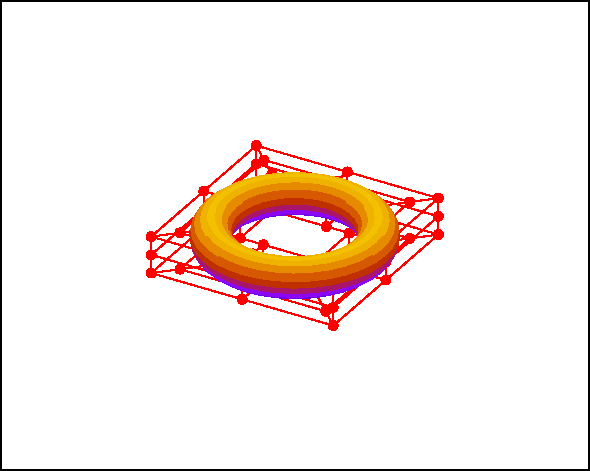
\includegraphics[height=4.6cm, trim=58 60 65 50, clip]{figures/torus.pdf}\hspace{1.5cm}
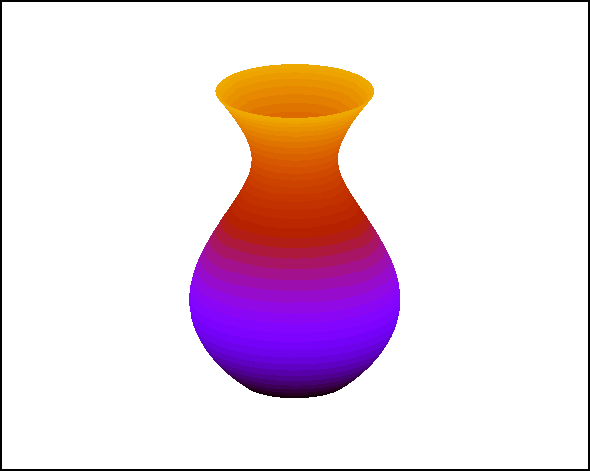
\includegraphics[height=4.6cm, trim=79 26 79 14, clip]{figures/vase.pdf}
\caption{Left: exact NURBS torus ($R=2$, $r=1/2$, degrees $2\times2$, $9\times9$ control net, shown). Right: surface of revolution interpolating eight measured profile points (Example 3). Both are drawn with \code{nurbs\_draw\_surface} and Maxima's \code{draw} package.}
\label{fig:surfaces}
\end{figure}

\paragraph{Validation} The regression suite \code{tests/rtest\_nurbs.mac} (Maxima's standard \code{rtest} format) contains 95 problems: textbook values (Example~2.3 of~\cite{PieglTiller1997}), symbolic identities (the circle satisfies $x^2+y^2=1$ on all four spans; Bézier bases equal Bernstein polynomials; $K=-1/(1+x^2+y^2)^2$ for $z=xy$), invariance under knot insertion, refinement, degree elevation, weight scaling and projective maps, Gauss--Bonnet on the sphere, torus and an ellipsoid, and symbolic-weight, bigfloat and export checks. All 95 pass in about 32\,s. Independently, \code{tests/crossval\_export.mac} exports 16 curves and surfaces to JSON, and \code{tests/crossval\_geomdl.py} re-evaluates them with geomdl~5.5.1. The maximum absolute difference over points, first and second derivatives and normals is $2.3\times10^{-13}$ (a second derivative of a refined rational curve); for points alone it is $8.9\times10^{-16}$. Knot insertion, refinement, degree elevation (compared in Bézier form) and Bézier decomposition give identical knot vectors and control points that agree to $1.8\times10^{-15}$. Table~\ref{tab:accuracy} lists representative accuracy checks.

\begin{table}[t]
\centering
\small
\begin{tabular}{@{}lc@{}}
\toprule
Check (\code{tests/accuracy\_table.mac}) & Max.\ abs.\ error \\
\midrule
Circle $x^2+y^2=1$, symbolic, 4 spans & 0 (exact) \\
Curve unchanged by insertion, refinement, elevation (exact) & 0 \\
Circle $r=3$: curvature $1/3$ (14 points) / length $6\pi$ & $1.7\times10^{-16}$ / $3.6\times10^{-15}$ \\
Projective invariance, rational cubic (11 points) & $8.9\times10^{-16}$ \\
Torus $K$ against the analytic value ($8\times10$ grid) & $1.8\times10^{-15}$ \\
Torus area $4\pi^2Rr$ / volume $2\pi^2Rr^2$ & $1.4\times10^{-12}$ / $4.5\times10^{-13}$ \\
Sphere $\iint K\,dA=4\pi$ / torus $\iint K\,dA=0$ & $3.7\times10^{-12}$ / $6.4\times10^{-16}$ \\
\bottomrule
\end{tabular}
\caption{Representative accuracy (double precision unless stated).}
\label{tab:accuracy}
\end{table}

\paragraph{Example 1: curvature at the singular poles of a NURBS sphere} (\code{examples/04\_torus.mac}). The rational sphere of revolution has singular points ($S_u\times S_v=0$) at its poles; \code{nurbs\_singular\_points} finds 18 singular grid nodes, all at $z=\pm1$. Near a pole both $EG-F^2$ and $LN-M^2$ in Eq.~\eqref{eq:KH} tend to zero, and their quotient suffers catastrophic cancellation. Fig.~\ref{fig:numerics}a shows $|K-1|$ on the unit sphere at parameter distance $\varepsilon$ from the pole. In double precision the error grows erratically; at $\varepsilon=10^{-9}$ the computed curvature is $-36.9$ instead of $1$. The same code, given a bigfloat copy of the sphere with \code{fpprec:50}, keeps the error below $1.5\times10^{-25}$ for every $\varepsilon\ge10^{-14}$, that is, at least 24 correct digits. Away from singular points the double results are reliable: the computed $K$ of the torus matches the analytic value to $1.8\times10^{-15}$ (Table~\ref{tab:accuracy}), and the ellipsoid with semi-axes $3,2,1$, obtained exactly by scaling the sphere, satisfies Gauss--Bonnet with an error of $-3.0\times10^{-6}$ ($4\times4$ quadrature cells per span), even though its curvature varies from $0.028$ to $2.25$.

\paragraph{Example 2: a design weight as a symbol} (\code{examples/06\_symbolic\_weight\_study.mac}). For the quadratic rational Bézier curve with control points $(-1,0),(0,1),(1,0)$ and weights $1,w,1$, \pkg{} returns the rational parametrisation; eliminating $t$ gives a conic with discriminant $64(w-1)w^2(w+1)$, so the curve is an ellipse for $w<1$, a parabola for $w=1$ and a hyperbola for $w>1$, the classical result of~\cite[Ch.~7]{PieglTiller1997}, here derived rather than quoted. The curvature at the apex is exactly $\kappa(1/2)=w$, and for $w=1/\sqrt2$ the package proves that $x^2+(y+1)^2-2\equiv0$. For a biquadratic Bézier patch over $[0,2]^2$ whose centre control point is raised to height~1 with weight $w$, \code{nurbs\_curvature\_sym} gives the height of the centre $w/(w+3)$, the Gaussian curvature there $K=w^2/4$ and the mean curvature $H=-w\sqrt{(w+3)^6}/\bigl(2(w+3)^3\bigr)=-w/2$, and Maxima confirms that $dK/dw>0$ for all $w>0$. The symbolic $K$ at $w=3$ coincides with the numerical evaluation of the corresponding patch (difference $0.0$). Fig.~\ref{fig:weight} plots the closed forms together with quantities that have no elementary closed form and are computed numerically (arc length and area).

\paragraph{Example 3: from measured profile to ParaView and 3D printing} (\code{examples/07\_scientific\_workflow.mac}). Eight measured points of a vase profile are interpolated by a cubic (centripetal parameters, LU solve, residual $4.4\times10^{-16}$) and revolved into an exact rational surface of degrees $2\times3$ with a $9\times8$ control net (Fig.~\ref{fig:surfaces}, right). On a $48\times40$ grid the shared helper gives $K\in[-3.672,\,1.018]$ and $H\in[-1.027,\,-0.135]$; 53.7\,\% of the points are elliptic and 46.3\,\% hyperbolic, and $K$ changes sign at the inflection of the profile (Fig.~\ref{fig:numerics}b). The lateral area is $21.2322$ and $\iint K\,dA=1.1192965$. Because the surface is an annulus ($\chi=0$), the Gauss--Bonnet theorem with boundary reduces, for a surface of revolution, to $\iint K\,dA=2\pi\,(r'(s_0)-r'(s_1))$, where $r'$ is the radial slope of the profile per unit arc length at the bottom and top. Evaluating the right-hand side from the profile gives $1.1192980$, a relative agreement of $1.4\times10^{-6}$ that validates the curvature field without any external library. Refining the surface in $v$ leaves it unchanged to $1.1\times10^{-16}$. The script ends by writing the surface to VTK (with $K$, $H$ and normals for ParaView), STL for 3D printing, OBJ and geomdl JSON.

\begin{figure}[t]
\centering
\begin{tikzpicture}
\begin{groupplot}[group style={group size=2 by 1, horizontal sep=2.2cm},
  width=0.43\linewidth, height=5.2cm, tick label style={font=\scriptsize},
  label style={font=\small}, legend style={font=\scriptsize}]
\nextgroupplot[xmode=log, ymode=log, x dir=reverse,
  xlabel={distance to the pole $\varepsilon$}, ylabel={$|K-1|$},
  ymin=1e-52, ymax=1e3, legend style={font=\scriptsize, at={(0.5,-0.32)}, anchor=north}, legend cell align=left,
  title={\small (a) unit sphere near a pole}]
\addplot[mark=*, mark size=1.4pt, red!75!black] table[x=eps, y=errdouble, col sep=comma] {figures/pole_sweep.csv};
\addlegendentry{double}
\addplot[mark=square*, mark size=1.4pt, blue!70!black] table[x=eps, y=errbfloat, col sep=comma] {figures/pole_sweep.csv};
\addlegendentry{bigfloat, 50 digits}
\nextgroupplot[xlabel={height $z$}, ylabel={$K$}, axis y line*=left,
  ymin=-4, ymax=1.5, title={\small (b) vase, along a meridian}]
\addplot[thick, blue!70!black] table[x=z, y=K, col sep=comma] {figures/vase_meridian.csv};
\addplot[dashed, gray, domain=0:3.5] {0};
\end{groupplot}
\begin{axis}[at={(group c2r1.south west)}, width=0.43\linewidth, height=5.2cm,
  axis x line=none, axis y line*=right, ymin=0, ymax=1.4,
  ylabel={profile radius $x$}, tick label style={font=\scriptsize},
  label style={font=\small}, xmin=0, xmax=3.5]
\addplot[thick, orange!80!black, densely dotted] table[x=z, y=x, col sep=comma] {figures/vase_meridian.csv};
\end{axis}
\end{tikzpicture}
\caption{(a) Error of the Gaussian curvature of the unit NURBS sphere at parameter distance $\varepsilon$ from a singular pole, same code in double and in 50-digit arithmetic (\code{figures/pole\_sweep.csv}). (b) Gaussian curvature (solid, left axis) and profile radius (dotted, right axis) along a meridian of the vase of Example~3; $K$ changes sign at the inflection of the profile (\code{figures/vase\_meridian.csv}).}
\label{fig:numerics}
\end{figure}

\begin{figure}[t]
\centering
\begin{tikzpicture}
\begin{groupplot}[group style={group size=2 by 1, horizontal sep=1.8cm},
  width=0.45\linewidth, height=5cm, xlabel={weight $w$}, xmode=log,
  log basis x=2, tick label style={font=\scriptsize}, label style={font=\small},
  legend style={font=\scriptsize, at={(0.5,-0.32)}, anchor=north}, legend cell align=left]
\nextgroupplot[ylabel={curve}, title={\small (a) rational quadratic arc}]
\addplot[thick, blue!70!black, domain=0.25:8, samples=60] {x};
\addlegendentry{$\kappa(1/2)=w$ (closed form)}
\addplot[only marks, mark=*, mark size=1.4pt, orange!80!black] table[x=w, y=length, col sep=comma] {figures/weight_study.csv};
\addlegendentry{arc length (numerical)}
\nextgroupplot[ylabel={patch}, ymode=log, title={\small (b) weighted biquadratic patch}]
\addplot[thick, blue!70!black, domain=0.25:8, samples=60] {x^2/4};
\addlegendentry{$K(\tfrac12,\tfrac12)=w^2/4$ (closed form)}
\addplot[only marks, mark=*, mark size=1.4pt, orange!80!black] table[x=w, y=area, col sep=comma] {figures/weight_study.csv};
\addlegendentry{area (numerical)}
\end{groupplot}
\end{tikzpicture}
\caption{Parametric study of a weight $w$ (Example~2). Lines: closed forms returned by \pkg; the numerical values of $\kappa$ and $K$ in \code{figures/weight\_study.csv} lie on them to all printed digits. Markers: arc length and area, which have no elementary closed form.}
\label{fig:weight}
\end{figure}

\paragraph{Performance} Table~\ref{tab:bench} compares mean times per call with geomdl (\code{tests/benchmark.mac}, \code{tests/benchmark\_geomdl.py}). Converting objects to floating point is the decisive optimisation: exact evaluation of the torus keeps $\sqrt2$ symbolic and makes the curvature computation about 33 times slower. In double precision \pkg{} is 26--62 times slower than geomdl in this run (36--50 times in an earlier run on the same machine, which indicates the run-to-run variability); \code{nurbs\_compile()} reduces the gap only partially (1.3--2.1 times), since much of the cost lies in Maxima's generic list arithmetic and simplification. Bigfloat (32 digits) costs 6--8 times double, which is affordable for the few evaluations where precision matters.

\begin{table}[t]
\centering
\small
\resizebox{\linewidth}{!}{% Generated from tests/benchmark.mac + tests/benchmark_geomdl.py (run of 2026-11-25);
% raw output in figures/benchmarks_run.md
\setlength{\tabcolsep}{4pt}
\begin{tabular}{@{}lrrrrrr@{}}
\toprule
Operation & exact & double & bigfloat & double + & geomdl & double / \\
 & & & (32 digits) & \code{compile} & & geomdl \\
\midrule
Curve point (circle)              & 0.42  & 0.26 & 1.66  & 0.12 & 0.0063 & 42$\times$ \\
Curve derivatives, order 2        & 0.94  & 0.90 & 5.10  & 0.66 & 0.015  & 62$\times$ \\
Surface point (torus)             & 0.92  & 0.56 & 4.04  & 0.43 & 0.012  & 47$\times$ \\
Surface derivatives, order 2      & 4.35  & 2.81 & 15.75 & 1.87 & 0.107  & 26$\times$ \\
$K$, $H$, $\kappa_1$, $\kappa_2$ (shared helper) & 100.0 & 3.00 & 22.5 & 1.91 & n/a & -- \\
$31\times31$ torus mesh with normals & -- & 1.26\,s & -- & -- & -- & -- \\
\bottomrule
\end{tabular}
}
\caption{Mean time per call in ms (each measurement loops for at least 1\,s). Maxima 5.46.0 (GCL), geomdl 5.5.1 on CPython 3.13; Intel Xeon @ 2.30\,GHz. geomdl has no surface-curvature routine. \todo{Repeat on the final machine, ideally also with Maxima on SBCL.}}
\label{tab:bench}
\end{table}

%% ===========================================================================
\section{Impact}
\label{sec:impact}

\pkg{} opens three kinds of use that, to our knowledge, were not possible with free software before.

\emph{New research questions.} Because the algorithms accept symbols, sensitivities of curvature, height or other differential quantities with respect to weights, control points or knots can be obtained in closed form and differentiated, as in Example~2. Because they accept bigfloats, reference values can be computed at degenerate points where floating-point libraries return noise (Example~1). Such high-precision values are useful as test oracles for other NURBS and isogeometric codes~\cite{Hughes2005,deFalco2011}.

\emph{Verification of algorithms and libraries.} Exact arithmetic turns ``agrees to $10^{-15}$'' into ``is identical'': the test suite proves that insertion, refinement and degree elevation leave a curve unchanged. During cross-validation, the same approach showed that applying geomdl's degree-elevation operation directly to a non-Bézier rational cubic with interior knots changed the curve by up to $0.336$ over 51 samples, whereas Algorithm A5.9 in \pkg{} leaves it unchanged; after Bézier decomposition both agree to $1.8\times10^{-15}$. The geomdl routine appears to be intended for Bézier input \todo{confirm in the geomdl documentation}; the practical lesson is that degree elevation of general NURBS should be validated, which exact arithmetic makes straightforward.

\emph{Teaching.} The algorithms are written in readable Maxima rather than hidden in a compiled kernel, and the results can be displayed both as formulas and as plots in the same wxMaxima notebook. The repository includes a Spanish-language notebook (\code{docs/programacion\_nurbs.wxm}) that explains how the package is programmed. The package has just been released and has no external users yet; we propose it as course material for students of symbolic computation, numerical analysis, computer-aided geometric design and differential geometry. Typical exercises are: deriving the basis functions with the Cox--de Boor recursion by hand and comparing them with the exact piecewise polynomials returned by \code{bspline\_basis\_piecewise}; proving that a rational quadratic curve is a conic and finding the weight that makes it a circle; checking that knot insertion and degree elevation do not change a curve, first exactly and then in floating point; and computing Gaussian and mean curvature of a surface and verifying the Gauss--Bonnet theorem numerically. Because Maxima and wxMaxima are free and run on Windows, Linux and macOS, such material can be used in universities without licence costs, and the Spanish notebook lowers the entry barrier for Spanish-speaking students. Evaluating this use in courses is a natural next step.

The package is deliberately not a CAD or meshing kernel. Its intended range is exact and symbolic analysis, high-precision reference computations, verification, teaching, and moderate meshes ($10^3$--$10^4$ points) exported for visualisation or fabrication. \emph{Limitations.} (i) Speed: floating-point evaluation is one to two orders of magnitude slower than a compiled or vectorised library (Table~\ref{tab:bench}), which limits practical meshes to about $10^4$ points. (ii) Expression growth: exact computations with irrational weights such as $\sqrt2/2$ (circles and quadrics) produce large radical expressions; \code{nurbs\_curvature\_sym} on such patches can exhaust Maxima's stack, so it is best used with rational or symbolic weights, and numerical or bigfloat evaluation is preferable otherwise. (iii) Scope: trimmed surfaces, surface--surface intersection, knot removal as a public operation, surface fitting and approximation, and import of CAD exchange formats (IGES, STEP) are not implemented; geometry is exchanged with other tools through the geomdl JSON format and mesh formats only. (iv) Singular points are detected with a relative tolerance on $|S_u\times S_v|$; very close to a singularity the floating-point classification depends on \code{nurbs\_tol}, and bigfloat evaluation is the reliable option (Example~1). (v) The package has been tested with Maxima~5.46.0 on GCL; other Lisp back-ends (SBCL, Clozure CL) are expected to work but have not been systematically tested.

%% ===========================================================================
\section{Conclusions}
\label{sec:conclusions}

\pkg{} brings the standard NURBS algorithms, a coherent differential-geometry layer and common exchange formats to the free computer algebra system Maxima, with a single code base for exact, symbolic, double and arbitrary-precision arithmetic. Cross-validation against NURBS-Python agrees to $2.3\times10^{-13}$, and the examples show results that floating-point libraries cannot give directly: curvature at a singular pole with at least 24 correct digits, and design sensitivities in closed form. Planned work includes trimmed surfaces, knot removal, surface fitting, faster evaluation through compiled kernels, testing on other Lisp back-ends, and a classroom evaluation of the package as teaching material.

%% ===========================================================================
\section*{CRediT authorship contribution statement}
\textbf{Ronald Paul Santamaria Silupu:} Conceptualization, Methodology, Software, Validation, Formal analysis, Visualization, Data curation, Writing -- original draft, Project administration. \textbf{Yheff Alexander Castillo Maza:} Conceptualization, Methodology, Software, Validation, Investigation, Writing -- original draft, Writing -- review \& editing. \textbf{Judith Keren Jimenez Vilcherrez:} Validation, Formal analysis, Writing -- review \& editing. \textbf{Rubén Teodoro Urbina Guzmán:} Methodology, Supervision, Writing -- review \& editing. \textbf{Victor Bernardo Sosa Gonzales:} Supervision, Resources, Writing -- review \& editing.

\section*{Declaration of competing interest}
The authors declare that they have no known competing financial interests or personal relationships that could have appeared to influence the work reported in this paper.

\section*{Declaration of generative AI and AI-assisted technologies in the manuscript preparation process}
During the preparation of this work the authors used Gemini (Google) and Claude (Anthropic) to assist with writing and testing parts of the software code, language refinement, structural clarity of the manuscript, and consistency of the mathematical notation. All code generated with these tools was reviewed by the authors and validated with the regression suite and the independent cross-validation described in Section~\ref{sec:examples}; the design of the package, the mathematical content and the scientific conclusions are the authors' own. After using these tools, the authors reviewed and edited the content as needed and take full responsibility for the content of the published article.

\section*{Data availability}
All data and scripts needed to reproduce the results are included in the software repository \url{https://github.com/ronaldpaul78/NURBS-Maxima}, archived at \todo{\url{https://doi.org/10.5281/zenodo.0000000}}: \code{tests/} (regression suite, accuracy table, cross-validation and benchmarks) and \code{docs/softwarex/figures/} (figure data).

\section*{Acknowledgements}
This research did not receive any specific grant from funding agencies in the public, commercial, or not-for-profit sectors. \todo{Add acknowledgements if any.}

\bibliographystyle{elsarticle-num}
\bibliography{references}

\end{document}
